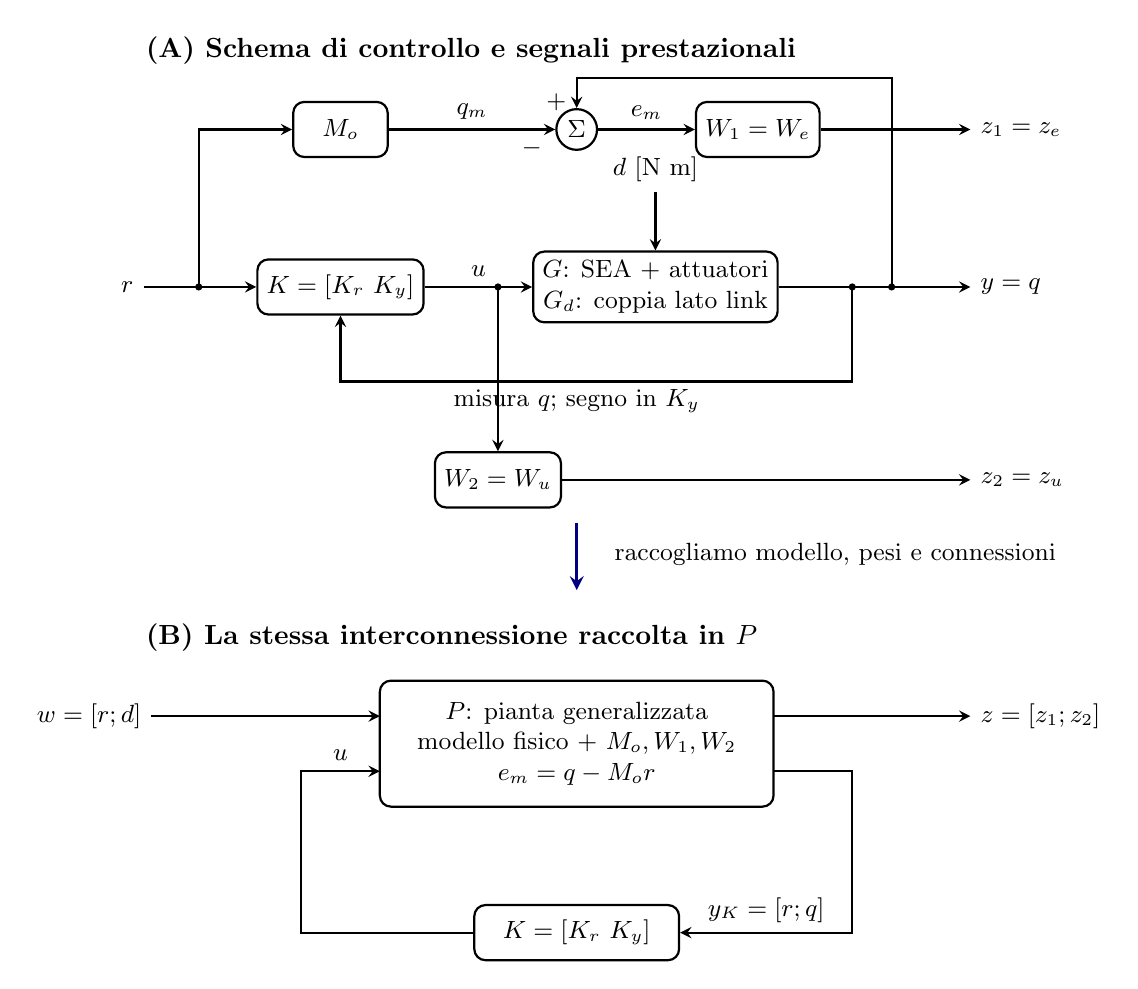
\begin{tikzpicture}[>=stealth,thick,
 b/.style={draw,rounded corners,align=center,minimum height=.7cm,minimum width=1.2cm},
 every node/.style={font=\small}]
\node[anchor=west,font=\bfseries] at (-2.6,4.8)
 {(A) Schema di controllo e segnali prestazionali};
\node[b] (k) at (0,1.8) {$K=[K_r\ K_y]$};
\node[b] (g) at (4,1.8) {$G$: SEA + attuatori\\$G_d$: coppia lato link};
\draw[->] (-2.5,1.8) node[left] {$r$} -- (k);
\draw[->] (k) -- node[above] {$u$} (g);
\draw[->] (g) -- (8,1.8) node[right] {$y=q$};
\draw[->] (6.5,1.8) -- (6.5,.6) -- (0,.6) -- (k.south);
\node at (3,.35) {misura $q$; segno in $K_y$};
\draw[->] (4,3) node[above] {$d$ [N m]} -- (g.north);
\node[b] (mo) at (0,3.8) {$M_o$};
\node[draw,circle,inner sep=2pt] (sum) at (3,3.8) {$\Sigma$};
\node[b] (w1) at (5.3,3.8) {$W_1=W_e$};
\draw[->] (-1.8,1.8) -- (-1.8,3.8) -- (mo);
\draw[->] (mo) -- node[above] {$q_m$} node[below,pos=.86] {$-$} (sum);
\draw[->] (7,1.8) -- (7,4.45) -- (3,4.45)
 -- node[left,pos=.8] {$+$} (sum.north);
\draw[->] (sum) -- node[above] {$e_m$} (w1);
\draw[->] (w1) -- (8,3.8) node[right] {$z_1=z_e$};
\node[b] (w2) at (2,-.65) {$W_2=W_u$};
\draw[->] (2,1.8) -- (w2.north);
\draw[->] (w2) -- (8,-.65) node[right] {$z_2=z_u$};
\fill (-1.8,1.8) circle (1.3pt);
\fill (2,1.8) circle (1.3pt);
\fill (6.5,1.8) circle (1.3pt);
\fill (7,1.8) circle (1.3pt);
\draw[->,very thick,blue!50!black] (3,-1.2) -- (3,-2.05);
\node[anchor=west] at (3.35,-1.6) {raccogliamo modello, pesi e connessioni};
\node[anchor=west,font=\bfseries] at (-2.6,-2.65)
 {(B) La stessa interconnessione raccolta in $P$};
\node[b,minimum width=5cm,minimum height=1.6cm] (p) at (3,-4)
 {$P$: pianta generalizzata\\modello fisico + $M_o,W_1,W_2$\\$e_m=q-M_or$};
\draw[->] (-2.4,-3.65) node[left] {$w=[r;d]$} -- (.5,-3.65);
\draw[->] (5.5,-3.65) -- (8,-3.65) node[right] {$z=[z_1;z_2]$};
\node[b,minimum width=2.6cm] (kb) at (3,-6.4) {$K=[K_r\ K_y]$};
\draw[->] (5.5,-4.35) -- (6.5,-4.35) -- (6.5,-6.4)
 -- node[above] {$y_K=[r;q]$} (kb.east);
\draw[->] (kb.west) -- (-.5,-6.4) -- (-.5,-4.35)
 -- node[above] {$u$} (.5,-4.35);
\end{tikzpicture}
